%%%%%%%%%%%%%%%%%%%%%%%%%%%%%%%%%%%%%%%%%%%%%%%%%%%%%%%%%%%%%%
%%%%		Informe de Máquinas DC
%%%%	Fecha	: Septiembre 2020
%%%%	Autor	: Luis Millan
%%%%	Correo	: lmillan131@gmail.com
%%%%
%%%%%%%%%%%%%%%%%%%%%%%%%%%%%%%%%%%%%%%%%%%%%%%%%%%%%%%%%%%%%%

\documentclass[11pt,letterpaper]{article}
\usepackage[activeacute,spanish]{babel}
\usepackage[utf8]{inputenc}
\usepackage[letterpaper,includeheadfoot, top=0.5cm, bottom=3.0cm, right=2.0cm, left=2.0cm]{geometry}
\renewcommand{\familydefault}{\sfdefault}
\usepackage{graphicx}
\usepackage{color}
\usepackage{hyperref}
\usepackage{amssymb}
\usepackage{url}
\usepackage{fancyhdr}
\usepackage{hyperref}
\usepackage{subfig}
\usepackage{listings}
\usepackage{mathrsfs,amsmath}
\lstset{language=C, tabsize=4,framexleftmargin=5mm,breaklines=true}

% =============== Inicio de Documento =============== 
\begin{document}
% =============== Portada =============== 
\newpage
\pagestyle{fancy}
\fancyhf{}
%\fancyhead[L]{ \includegraphics[scale=0.9]{logodgf.jpeg} }
\vspace*{6cm}
\begin{center}
\Huge  {Canalizaciones y Distribución}\\
\vspace{1cm}
\end{center}
\vfill
\begin{flushright}
\begin{tabular}{ll}
Autor: & Luis E. Millán U.\\
Profesor: & Ing. Jorge Crespo\\
& \today\\
& Caracas, Venezuela.
\end{tabular}
\end{flushright}

% =============== Encabezado y pie de Pagina ===============
\newpage
\pagestyle{fancy}
\fancyhf{}
%Encabezado
\fancyhead[L]{\rightmark}
\fancyhead[L]{\small \rm \textit{Sección \rightmark}}
\fancyhead[R]{\small \rm \textbf{\thepage}}
%Pie 
\fancyfoot[L]{\small \rm \textit{Br. L. Millán}}
\fancyfoot[R]{\small \rm \textit{Canalizaciones y Distribución}}
\renewcommand{\sectionmark}[1]{\markright{\thesection.\ #1}}
\renewcommand{\headrulewidth}{0.5pt}
\renewcommand{\footrulewidth}{0.5pt}
\tableofcontents
%\listoffigures
%==========================================%
%  MOTORES
%==========================================%
\newpage
\section{Información General}
\subsection{Objetivos}
\subsubsection{Objetivo Principal:}
Adquirir conocimientos y herramientas necesarias para realizar diseños e implementaciones de proyectos de canalizaciones eléctricas y distribución.
\subsubsection{Objetivos Especificos:}
\begin{itemize}
	\item Aprender la distribución de la electricidad desde la acometida hasta los circuitos ramales.
	\item Proteger los ciscuitos y balancear los tableros.
	\item 3.
\end{itemize}
\subsection{Formato de Clases}
La dinamica de las Clases será tipo Forochat, los dias Lunes y Miercoles desde las 8:00 a las 10:00, las dudas seran solventadas durante la hora de clase a través del chat privado, exceptuando aquellas dudas que se considere muy importante podra ser planteada en el chat grupal.
\subsection{Metodo de Evaluación}

\begin{itemize}
	\item \textbf{Parcial 1:} $30\%$
	\item \textbf{Parcial 2:} $20\%$
	\item \textbf{Proyecto 1:} $30\%$ (Individual)
	\item \textbf{Proyecto 2:} $15\%$ (Individual)
	\item \textbf{Asignaciones:} $5\%$
	
	
\end{itemize}
\section{Clases}
\subsection{Clase 1 Lunes 23/11/2020}
\textbf{Introducción}
\subsubsection{Partes de un Proyecto:}
\begin{itemize}
	\item \textbf{1} introducción del proyecto a desarrollar. El objetivo y lo que se necesita.

	\item \textbf{2} ubicación - condiciones ambientales (características del terreno; altitud; temperatura; nivel ceraunico; valores de resistividad del suelo)

	\item \textbf{3} características de la instalación (alta/media/baja; si es un centro comercial/colegio/residencia, etc)
 
	\item \textbf{4} alcance: elementos que se deben desarrollar para cumplir los objetivos del proyecto)

	\item \textbf{5} Referencias (nacionales e internacionales) 

	\item \textbf{6} criterios en base a las referencias 

	\item \textbf{7} cálculos.

	\item \textbf{8} especificaciones (materiales al detalle, altura, posición, ubicación, tipo de tubería, etc).

	\item \textbf{9} planos

	\item \textbf{10} cómputos (indicar cantidades de lo que se necesita)

	\item \textbf{11} Partida (Norma covenin 2000)

	\item \textbf{12} Análisis de precios unitarios (APU)

	\item \textbf{13} Costos - Precio general de la obra
\end{itemize}

\subsubsection{Alcances}
Los alcances pueden ser generales o de cargas especiales:

\begin{itemize}
	\item Fuerza: bomba de agua, portón eléctrico, ascensor, A.A, Cerco eléctrico.
	\item Iluminación: Interior (residencial, comercial, oficinas, fábricas, accesos, estacionamientos),	exterior (vial, fachada, recreación, estacionamiento, peatonal, de seguridad), emergencia, deportiva, arquitectónica.
	\item tomas de corriente de uso general.
	\item cargas o salidas especiales.
	\item Sistemas de intercomunicación.
	\item Sistemas de tv por cable.
	\item Sistemas de puesta a Tierra
	\item sistema de teléfono.
	\item sistema de protección contra incendios.
	\item Sistema de protección contra descargas atmosféricas.
	\item Sistemas de vigilancia y seguridad.
\end{itemize}

\textbf{Nota:} Es importante las referencias en los proyectos, eso permite estar en norma respecto al país donde se desarrolle el proyecto y en caso que no exista regulación siempre tendrán las normas internacionales, nosotros nos regimos por el Código Eléctrico Nacional, el cual se basa en el NFPA de EEUU.\\
Actualmente existen normativas para cada etapa de los proyectos, entre las nacionales tenemos: Fondonorma / Covenin y CEN - Fondonorma 200.\\
Ej: Rayos - Fondonorma 599; Tensiones normalizadas - Fondonorma 159\\

Las internacionales son: IEEE, IEC, NFPA.
\subsection{Clase 2 Miércoles 25/11/2020}
\subsubsection{Selección de Conductores}
Criterio para la selección de Conductores:
\begin{itemize}
	\item \textbf{1} capacidad de corriente
	\item \textbf{2} caída de tensión.
	\item \textbf{3} capacidad de cortocircuito.
	\item \textbf{4} nivel de tensión.
	\item \textbf{5} fluctuaciones de tensión.
	\item \textbf{6} ambiente de instalación
\end{itemize}
\textbf{Nota:} La conexión en hogares viene de un banco de transformadores local a un elemento de protección o breaker y
 finalmente a los diferentes tableros que alimentan los circuitos.\\
 
\textbf{Nota:} Intentar evitar empalmes, cada empalme es un punto de posible sobrecalentamiento.\\

\textbf{Nota:} La ventaja del aluminio sobre el cobre es basicamente su precio y el peso y las desventaja es que el cobre tiene una mayor capacidad para transportar corriente.\\
 
La primera característica a tomar en cuenta es la clasificación de los calibres de los cables (AWG/kcmil), desde el cable 18 hasta el 0000 (4/0) se denota AWG, en adelante se utiliza kcmil.\\

En baja tensión en aspectos residenciales normalmente se utilizan:

\begin{itemize}
	\item Cable 18 para control.
	\item Cable 12 tomas e iluminación.
	\item Cable 10 aires y cargas especiales.
	\item Cable 8 (secadoras, aires y cargas especiales)
	\item Cable 6 (acometidas)
\end{itemize}

\textbf{Nota:} Es importante la chaqueta según el ambiente en el que se vaya a trabajar. Existen chaquetas que soportan intemperie, agua, aceite, humedad, etc. Algunas chaquetas como la ttu y la thhn son robustas para evitar su fractura al ser cableadas o pasadas por tubos.\\

\textbf{Nota:} Cuando la temperatura del cable supera el límite permisible el aislante comienza a derretirse, si es fase activa es muy probable que haga contacto con otro cable o tubería y ¡EXPLOTA EL CABLE!\\

\textbf{Nota Secreto:} De manera general los fabricantes diseñan los cables cuidando un margen de seguridad. A los valores vistos normalmente el cable soporta hasta un 15$\%$ por encima de su valor.\\

Tenemos que considerar la temperatura ambiente, no es lo mismo dejar un cable a la intemperie en Maracaibo, en Mérida o en caracas, para una temperatura entre 26-30° el factor es 1, para Maracaibo que está como entre 36-40 (0,82).

\textbf{Nota:} De manera general se recomienda siempre trabajar con tres conductores portadores de corriente. Sin embargo, hay ocasiones en que hay que añadir una 4ta fase. Al agregar la 4ta fase, las características del conductor se reducen un 80$\%$ cómo lo establece la tabla 310.15\\

\begin{figure}[ht!]
	\centering
	\fbox{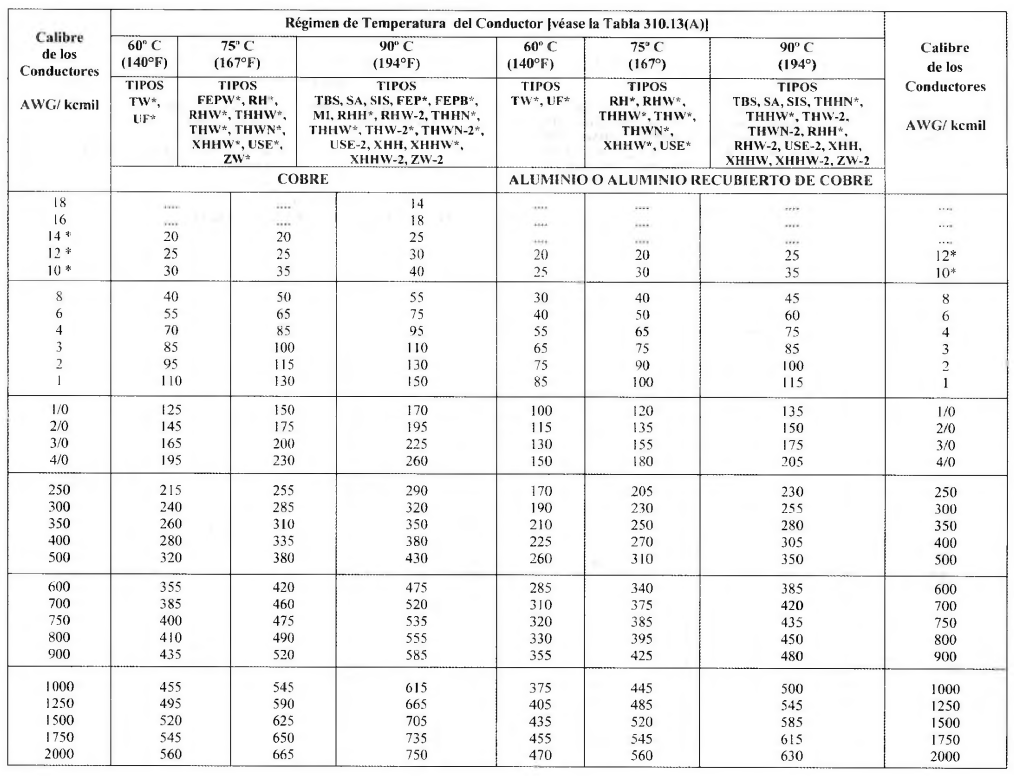
\includegraphics[scale=0.4]{310.16.png}}
	\caption{Ampacidades Admisibles de los Conductores Aislados para tensiones nominales (310.16)}
\end{figure}

\begin{figure}[ht!]
	\centering
	\fbox{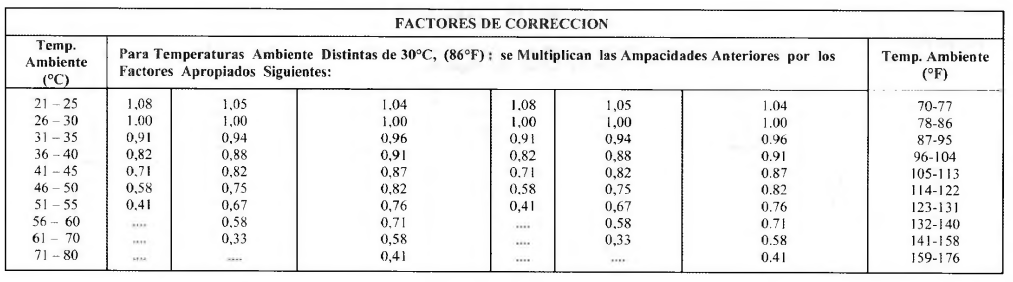
\includegraphics[scale=0.4]{310.16_correcciones.png}}
	\caption{Factor de Corrección para 310.16}
\end{figure}

\section{Asignaciones}
\subsection{Asignación 1 Miercoles 25/11/2020}
\textbf{Niveles de Tensión en Venezuela}
Segun el informe publicado el 16 de julio del 2020 con titulo: "INFORME DE COMISIÓN DE TRANSMISIÓN ELÉCTRICA", del Portal de Asociación Venezolana de Ingenieros Electricistas, Mecánicos y Profesiones Afines (AVIEM), los niveles de tensión en venezuela son: 69 kV; 115 kV; 138 kV; 230 kV; 400 kV y 765 kV.

Portal: \url{https://aviem.org/informe-de-comision-de-transmision-electrica/#:~:text=Los%20niveles%20de%20tensi%C3%B3n%20utilizados,400%20kV%20y%20765%20kV.}


\subsubsection{Retroalimentación}
\textbf{Nota:} Normalmente todos los centros comerciales realizan la distribución en 480V y cada local tiene un trx para tener nuestro servicio 208/120, esto facilita la alimentación de los chiller, ascensores y la distribución de la energía con una mayor eficiencia.\\

\subsection{Asignación 2 Lunes 30/11/2020}
\textbf{Tipos de Tableros de Distribución, Cantidad de Circuitos y Características y Plano de Casa}

	Los tableros eléctricos prácticamente son armazones metálicos que se utilizan para proteger a todos los componentes de mando y de control de cualquier sistema eléctrico, ya sea desde un circuito básico de un hogar hasta los componentes de uno más complejo como el de una máquina industrial.

\begin{figure}[ht!]
	\centering
	\fbox{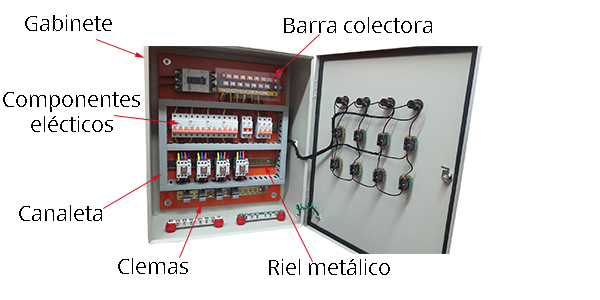
\includegraphics[scale=2]{Partes-tablero.jpg}}
	\caption{Partes de un Tablero}
\end{figure}
\subsubsection{Tipos de Tableros}
\begin{itemize}
	\item \textbf{Panel de Distribución para Circuitos Ramales de Alumbrado y de Artefactos}\\
	 Un panel de distribución para circuitos ramales de alumbrado y de artefactos es aquel que tiene más de un 10 por ciento de sus dispositivos de protec­ción de sobrecorriente de 30 amperios o menos protegiendo circuitos ramales de alumbrado y de artefactos.
	 
	\item \textbf{Panel de Distribución de Potencia}\\
 Un panel de distri­bución de potencia es aquel, que tiene el 10$\%$ o menos de sus dispositivos de protección de sobrecorriente protegiendo circuitos ramales de alumbrado y de artefactos.
 
	\item \textbf{Tablero Eléctrico para Uso en Viviendas}\\
 Un tablero eléctrico para uso en viviendas es similar a un panel para alumbrado y artefactos, pero de máximo 250 voltios y equipado exclusivamente con interruptores automáticos en caja moldeada del tipo insertable.
 
 	\item \textbf{Tablero de Control Industrial} U ensamble de dos o más componentes consistente de uno de los siguientes:
 	\begin{enumerate}
 		\item Solamente componentes de circuitos de potencia, tales como controladores de motores, relés de sobrecarga, suiches y seccionadores con fusibles e interruptores automáticos.
 		
 		\item Solamente componentes de circuitos de control, tales como pulsadores, luces pilotos, selectores, temporiza- dores, suiches, relés de control, etc.
 		
 		\item Una combinación de componentes de circuitos de potencia y de control.
 	\end{enumerate}
 	Esos componentes, juntos con el cableado y los terminales, están montados sobre o dentro de una envolvente o montados sobre un panel auxiliar. El tablero de control industrial no incluye los equipos controlados.
\end{itemize}
\subsubsection{Circuitos Ramales}
Los circuitos ramales comprendidos en esta Sección se clasificarán de acuerdo con la capacidad de corriente nominal o el máximo valor de ajuste permitido del dispositivo de sobrecorriente. La clasificación de los circuitos ramales que no sean individuales será de 15,20, 30, 40 y 50 A. Cuando por cualquier razón se utilicen conducto­res de mayor capacidad, la capacidad nominal o ajuste del dispositivo de sobrecorriente especificado determinará la clasificación del circuito.

\begin{figure}[ht!]
	\centering
	\fbox{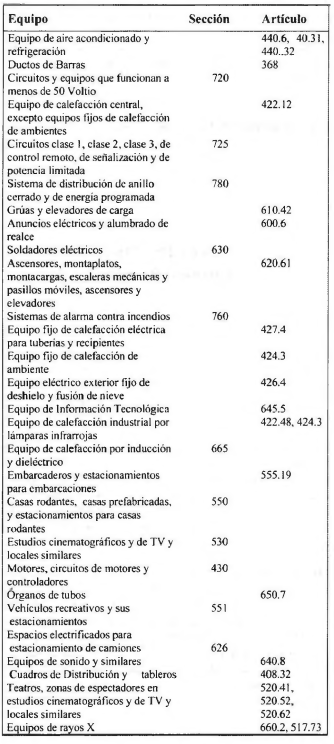
\includegraphics[scale=0.7]{210.2.png}}
	\caption{Circuitos Ramales para uso específico}
\end{figure}

\newpage
\textbf{Circuitos Ramales Necesarios} Los circuitos ramales para iluminación y aparatos, incluyendo los aparatos operados con motor serán provistos para suministrar las cargas calculadas según el Cálculo de Cargas del Circuito Ramal (220.10). Adicionalmente, los circuitos ramales serán provistos para cargas específicas no cubiertas por dicho cálculo donde sea requerido en cualquier parte de este Código y para cargas para unidades de vivienda según el Cálculo de Cargas del Circuito Ramal (220.10).
\begin{itemize}
	\item \textbf{Número de Circuitos Ramales} El número mínimo de circuitos ramales se determinará a partir de la carga total calculada y del tamaño o capacidad de los circuitos utilizados. En todas las instalaciones, el número de circuitos será el adecuado para alimentar la carga servida. En ningún caso, la carga de un circuito excederá la máxima especificada en la sección de Cargas Máximas (220.18).

	\item \textbf{Carga Proporcionalmente Repartida Entre los Circui­tos Ramales} Cuando la carga se calcula con base a voltioamperios por metro cuadrado, el sistema de cableado resultante, incluyendo los tableros para los circuitos ramales se proveerán para alimentar como mínimo la carga calculada. Esta carga será proporcionalmente repartida dentro de los circuitos ramales para salidas múltiples en los tableros. Los elementos de protecciones de los circuitos ramales y circuitos serán requeridos únicamente para servir las cargas conectadas.

	\item \textbf{Unidades de Viviendas}
		\begin{enumerate}
			\item \textbf{Circuitos Ramales para Pequeños Aparatos} En adición al número de circuitos ramales requeridos en otros sitios de este Artículo, dos o mas circuitos ramales de 20 A serán provistos para los tomacorrientes especificados en la seccion de Salidas para Tomacorrientes en Unidades de Vivienda (210.52).
			\item \textbf{Circuitos Ramales para Lavanderías} En adición al número de circuitos ramales requeridos en otros sitios de este Artículo, por lo menos un circuito ramal adicional de 20 A será provisto para el (los) tomacorriente(s) especifícado(s) en la seccion de Salidas para Tomacorrientes en Unidades de Vivienda (210.52). Este circuito no tendrá otras salidas.
			\item \textbf{Circuitos Ramales de Salas de Baño} En adición al número de circuitos ramales requeridos en otros sitios de este Artículo, al menos un circuito ramal de 20 A será provisto para el (los) tomacorriente(s) de la sala de baño. Este circuito no tendrá otras salidas.
		\end{enumerate}
\end{itemize}
\subsubsection{Retroalimentación}
\end{document}
